\begin{frame}

\begin{columns}[onlytextwidth]
    \begin{column}{0.45\textwidth}
    	\textbf{Improvements for electromagnetic interactions:}
    	\begin{itemize}
    		\item Inclusion of $\gamma \to \text{Hadrons}$ \\(Photohadronic interaction)
            \begin{itemize}
                \item[$\rightarrow$] Relevant for very-high energies
            \end{itemize}
    		%\item Sampling of deflection angles for bremsstrahlung photons
    		\item Inclusion of the photoeffect
            \begin{itemize}
                \item[$\rightarrow$] Relevant for low energies
            \end{itemize}
            \item Inclusion of $\gamma \to \mu^+ \mu^-$
            \begin{itemize}
                \item[$\rightarrow$] Relevant signatures (source of $\mu$-pairs in electromagnetic showers)
            \end{itemize}
    	\end{itemize}

    	%\hspace{10pt} $\Rightarrow$ More about this later!

    \end{column}
    \begin{column}{0.55\textwidth}

    \begin{figure}
    	\centering
        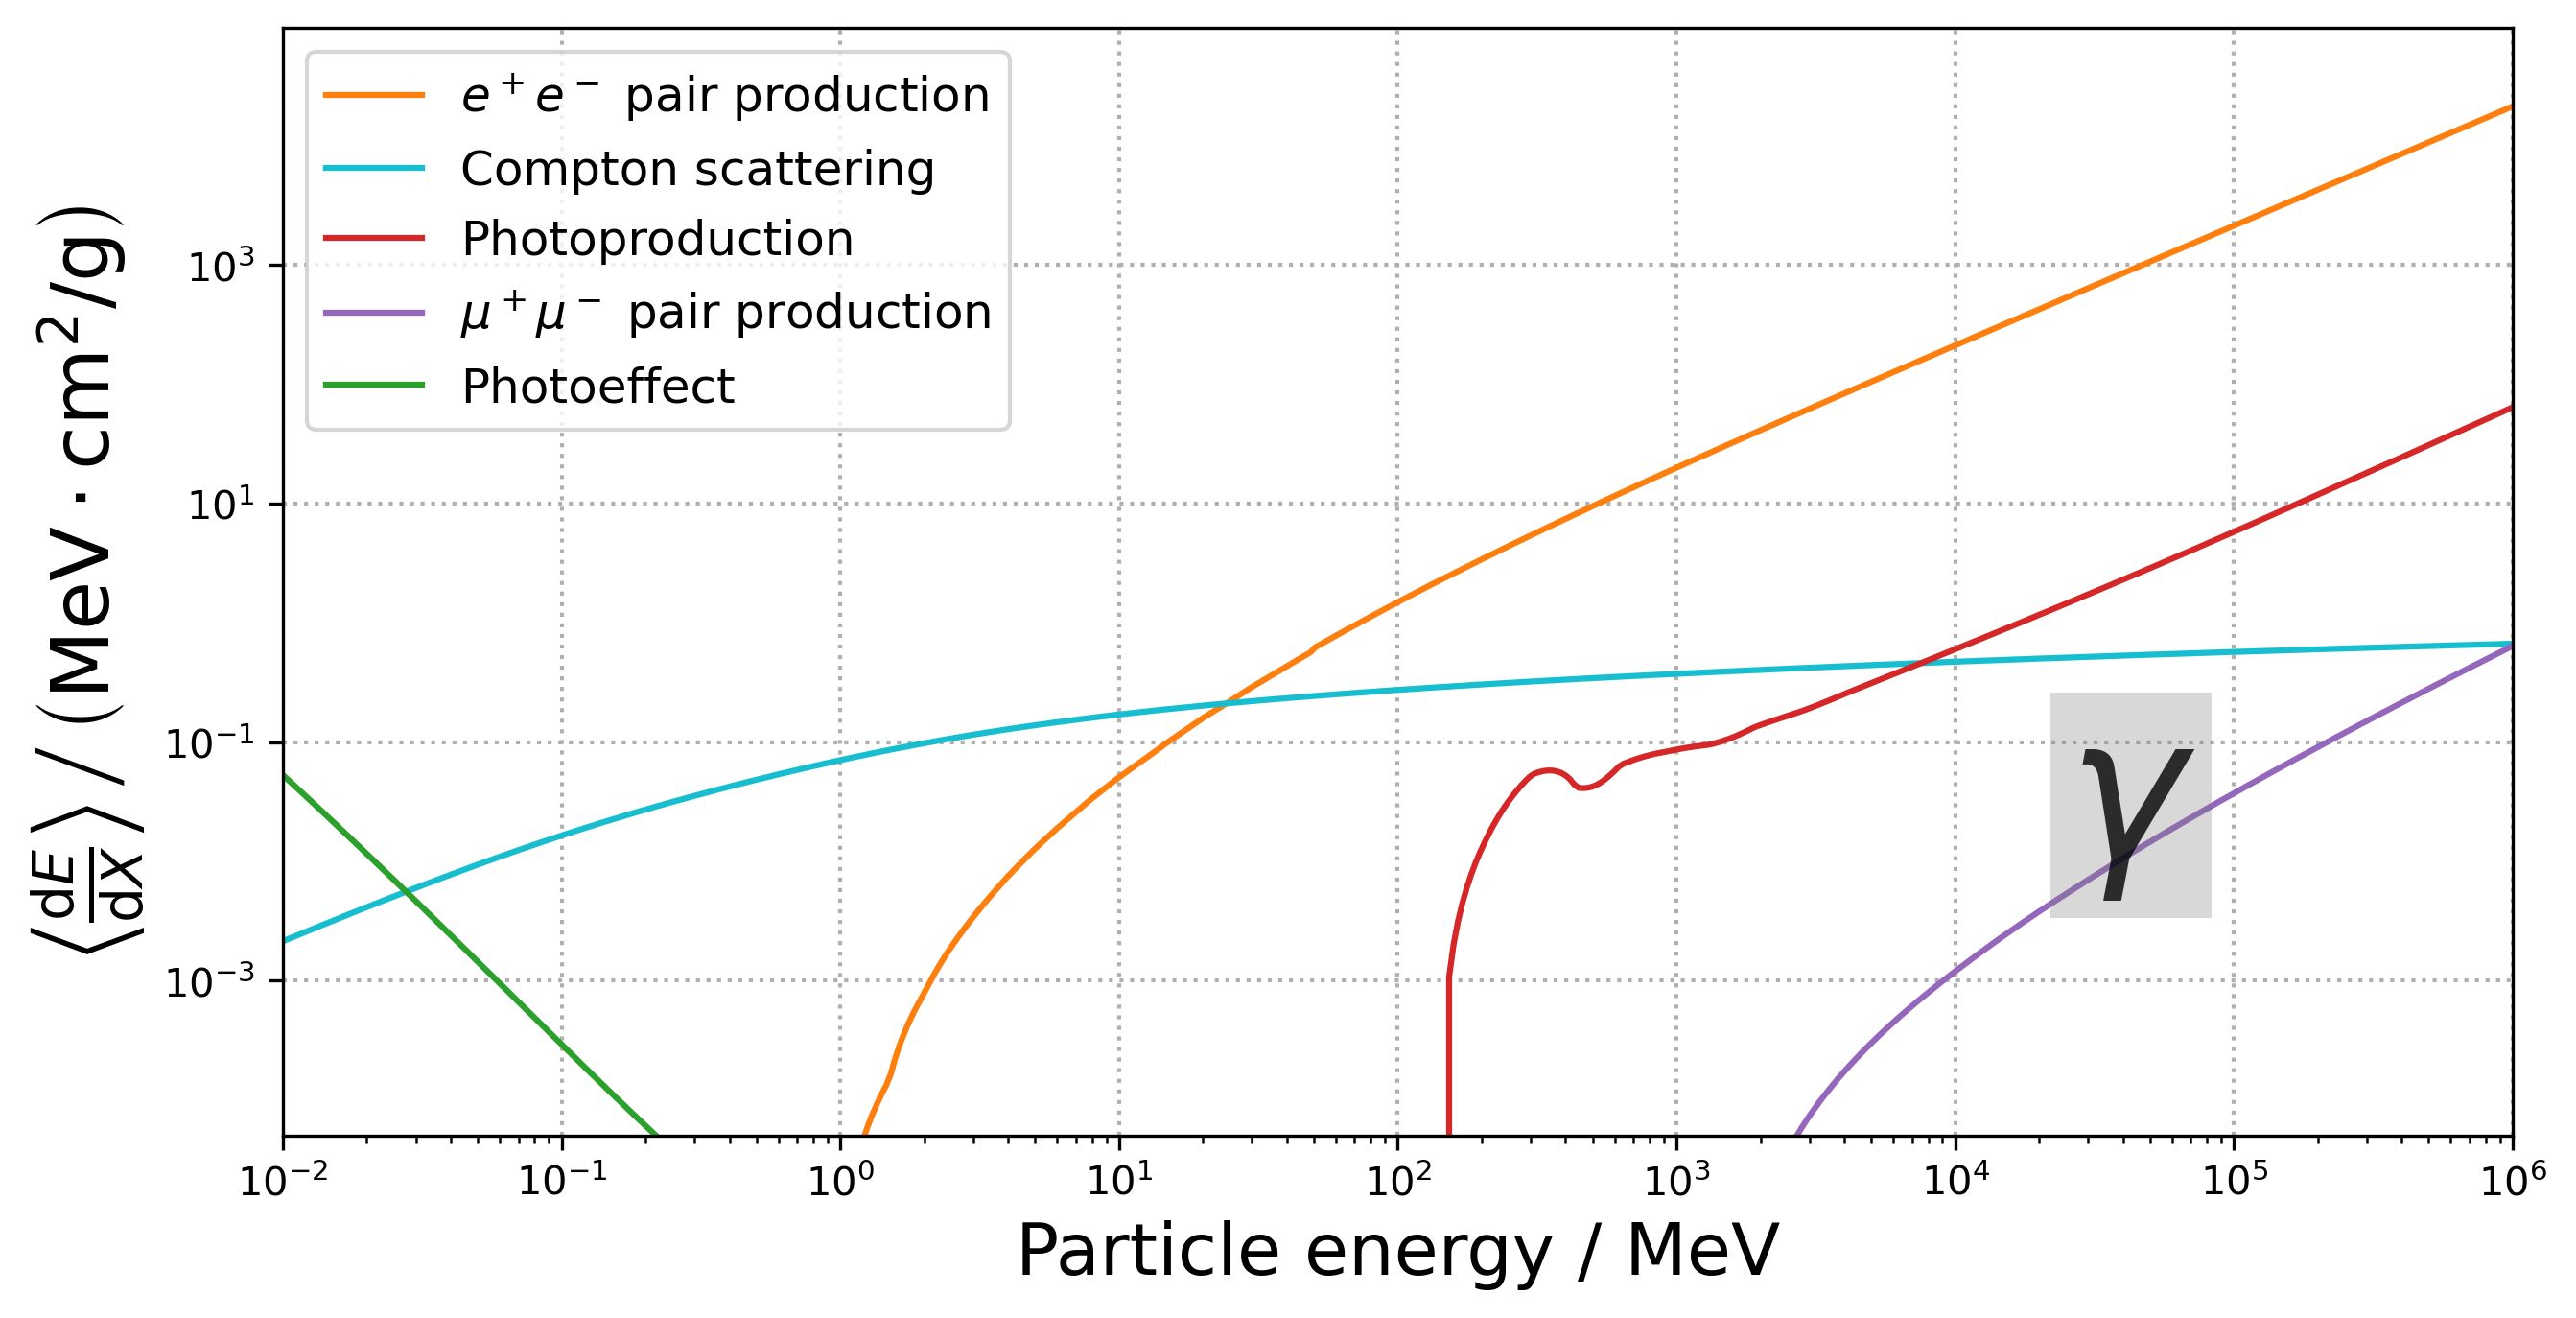
\includegraphics[width=0.9\textwidth]{plots/photon_dEdx.png}
    \end{figure}
    \vspace{-3mm}
    \begin{figure}
        \centering
        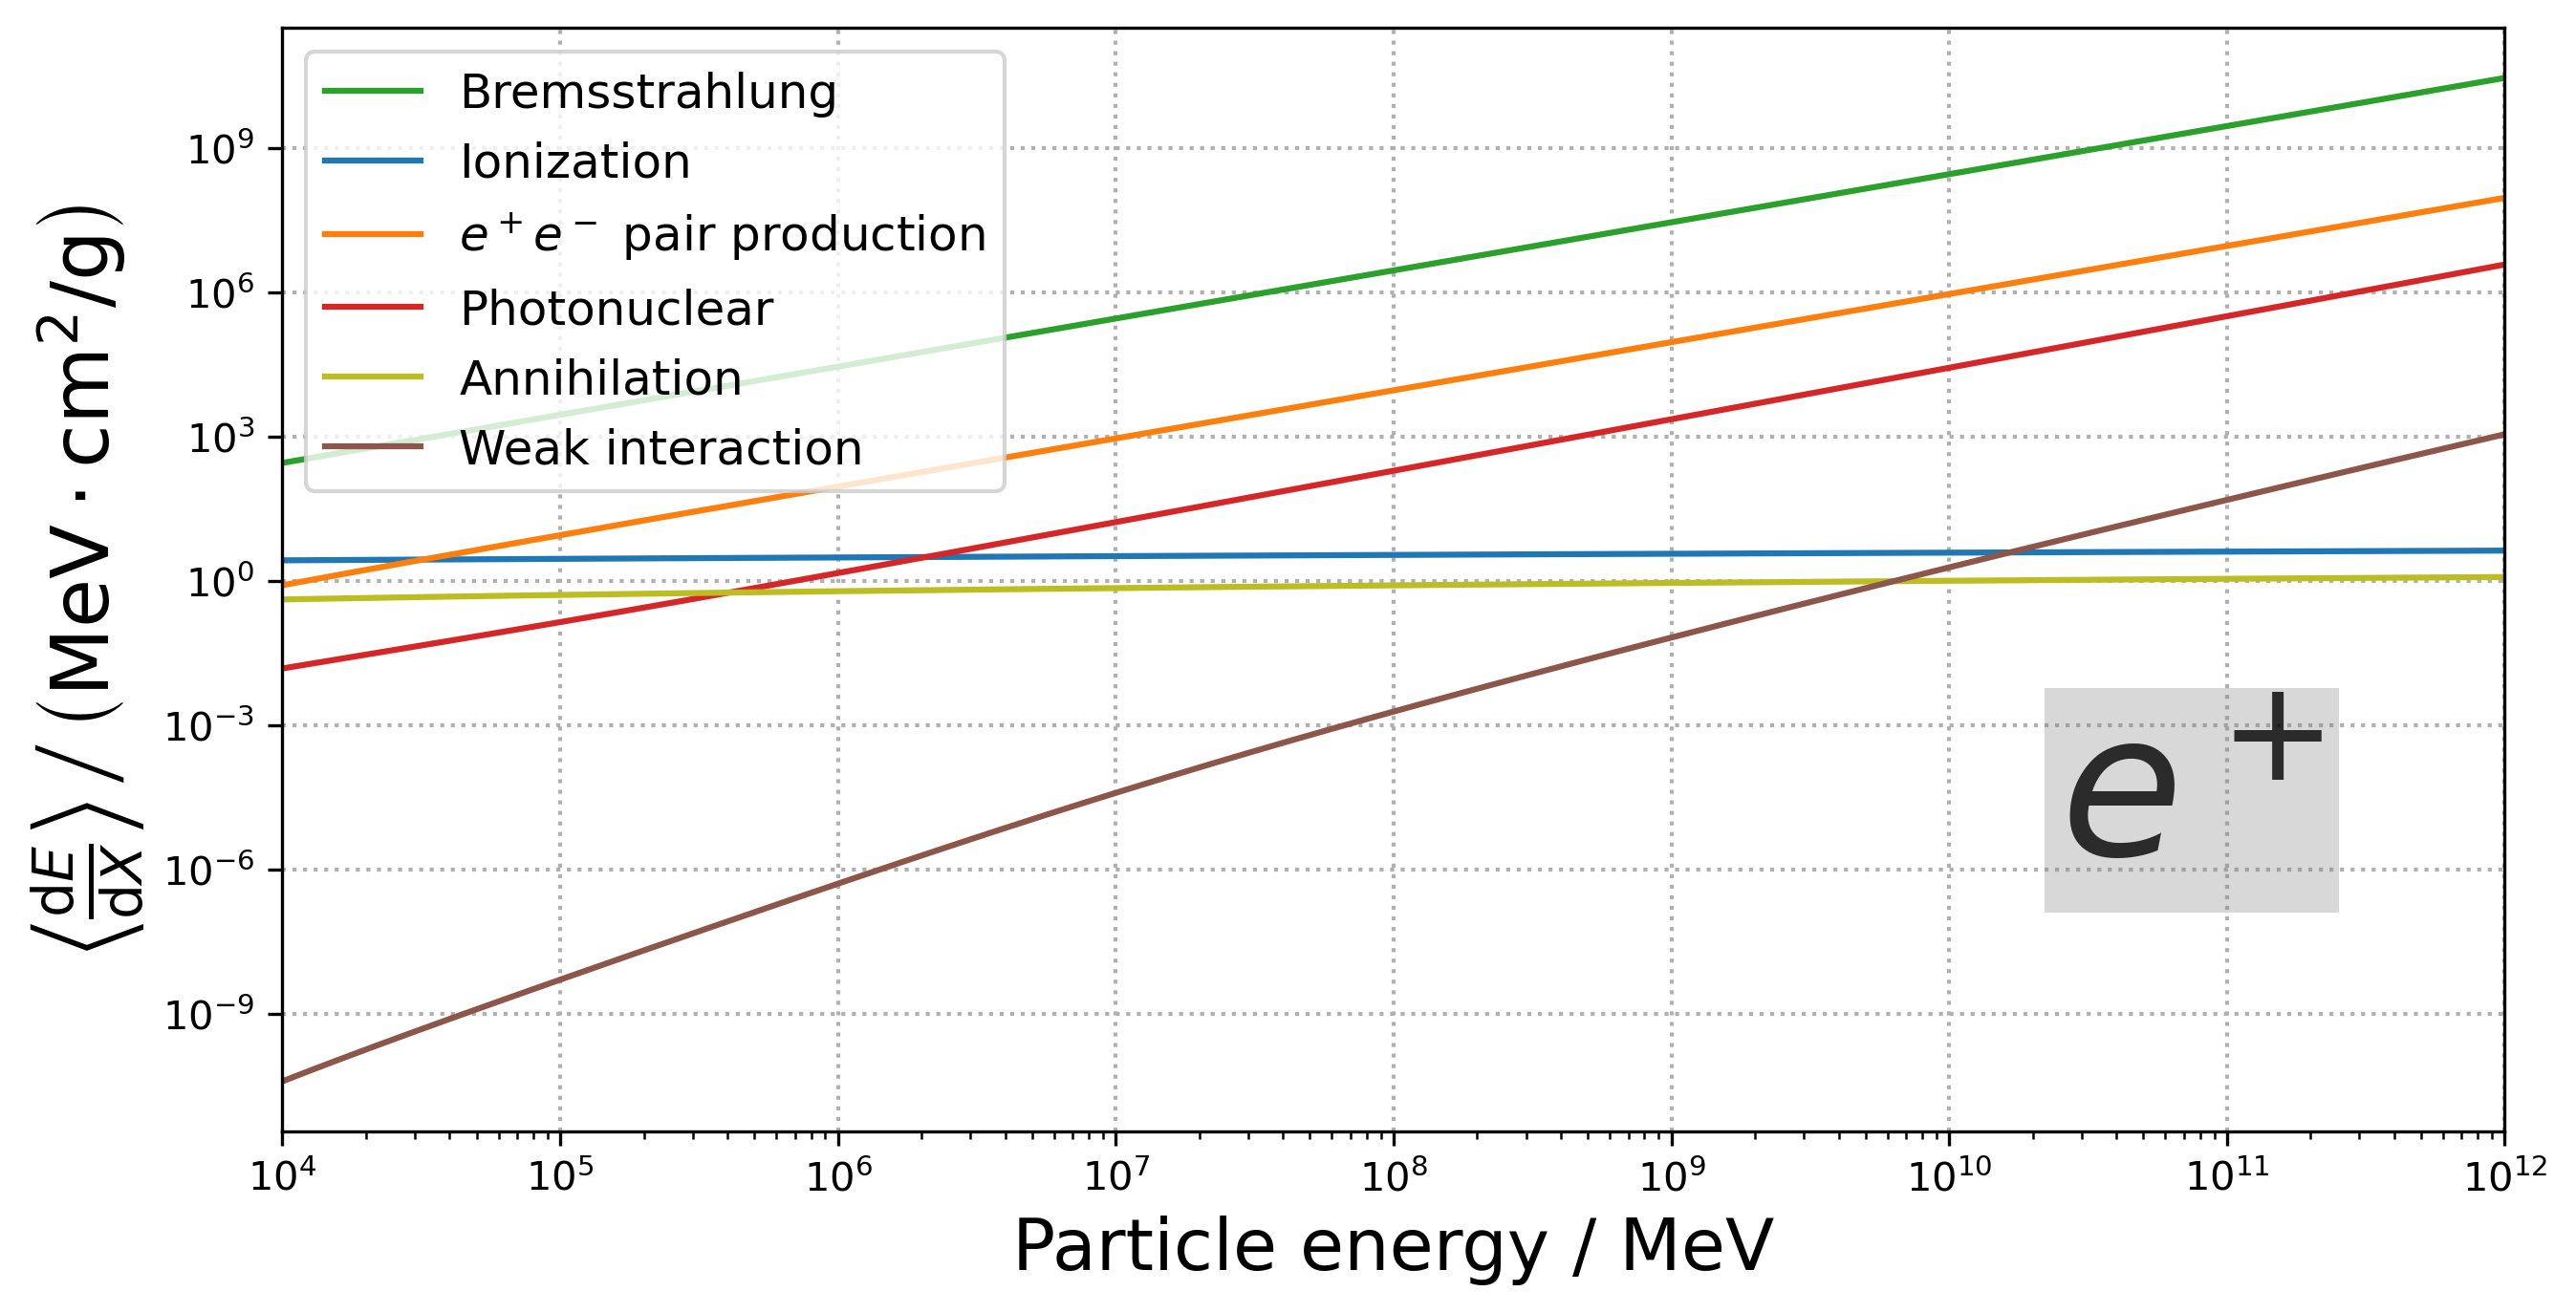
\includegraphics[width=0.9\textwidth]{plots/positron_dEdx.png}
    \end{figure}

    \end{column}
\end{columns}

\end{frame}



\begin{frame}[c]
    \begin{columns}[onlytextwidth]
    \begin{column}{0.45\textwidth}
        \textbf{Analysis of muon deflections}
        \begin{itemize}
            \item The main source of muon deflections is multiple scattering (scattering in continuous losses)
            \item However, deflection can also occur in individual, highly-stochastic interactions
            \begin{itemize}
                \item[$\rightarrow$] Both effects are implemented in PROPOSAL
            \end{itemize}
            \item We performed comparisons of muon deflections in PROPOSAL with other Monte Carlo tools (\textsc{Geant4}, MUSIC) and data
            \begin{itemize}
                \item[$\rightarrow$] We found them to be in good agreement
            \end{itemize}
        \end{itemize}

    \end{column}
        \begin{column}{0.55\textwidth}

            \begin{figure}
              %\vspace{-9pt}
              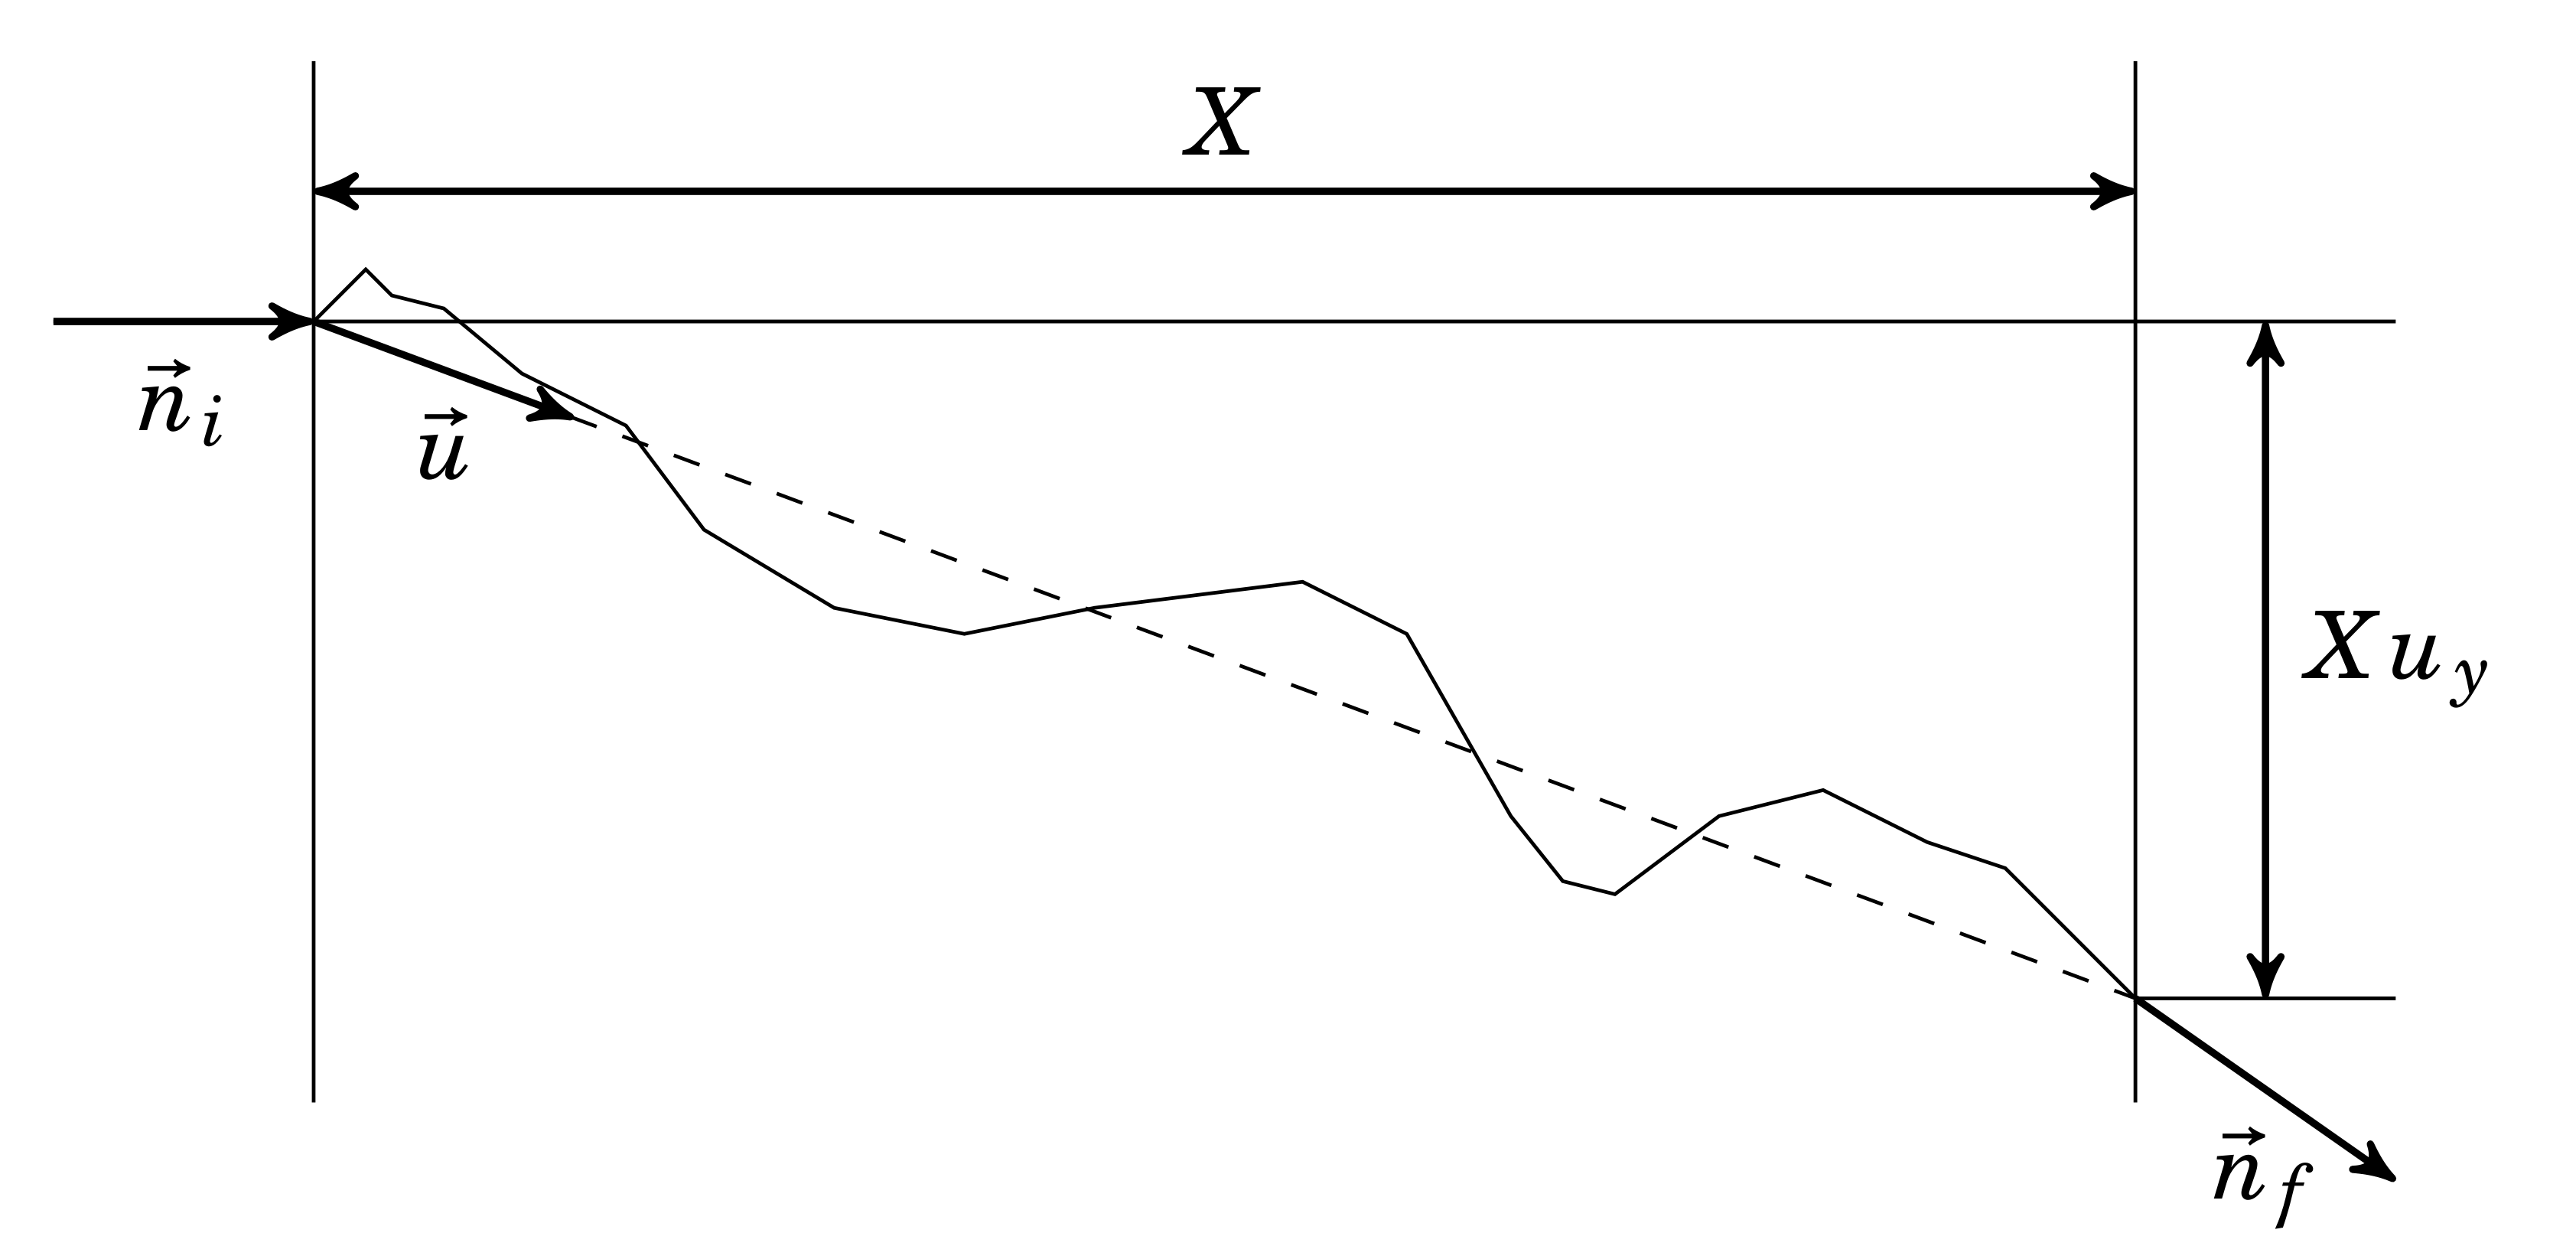
\includegraphics[width=0.8\linewidth, keepaspectratio]{plots/multiple_scattering_dunsch.png}
              \captionsetup{justification=centering}
              %\caption*{Paper by P.~Gutjahr et al., submitted to EPJ C \\(available as \href{https://arxiv.org/abs/2208.11902}{arXiv:2208.11902})}
            \end{figure}
        \vspace{3pt}
        \begin{figure}



            \begin{tikzpicture}[scale=0.7, every node/.style={scale=0.7}]
                \centering

                \coordinate (start) at (-1,0);
                \coordinate (kink) at (1.8, 0);
                \coordinate (end) at (4.5, 0.8);
                \coordinate (continue) at (4.5, 0);



                \draw [black, line width=0.6mm] (start) -- node[above] {$\mu$}  (kink);
                \draw [->, black, line width=0.6mm] (kink) -- node[above] {$\mu^\prime$}  (end);
                \draw [black, dashed, line width=0.2mm] (kink) -- (continue);

                \fill [red] (kink) circle (0.15) node[label=below: $\substack{\text{stochastic} \\ \text{interaction}}$]{};

                \pic [draw, "$\theta$", angle eccentricity=0.7, angle radius=2cm] {angle = continue--kink--end};

            \end{tikzpicture}
        \end{figure}  

        \end{column}
    \end{columns}
\end{frame}




\begin{frame}[c]
    \begin{columns}[onlytextwidth]
    \begin{column}{0.45\textwidth}
        \textbf{Analysis of muon deflections}
        \begin{itemize}
            \item We have investigated the influence of muon deflections on directional resolutions based on PROPOSAL simulations
            \item We performed simulations of muons with identical initial energies, and plotted the accumulated muon deflections for different final energies
            \begin{itemize}
                \item[$\rightarrow$] Accumulated deflection primarily depends on the final muon energy (independent of initial energy)
                \item[$\rightarrow$] We can see a potential impact of muon deflections on the angular regolution of KM3NeT at energies $E_\text{f} \leq \SI{1}{\tera\electronvolt}$
            \end{itemize} 
        \end{itemize}

    \end{column}
        \begin{column}{0.55\textwidth}
    		\begin{figure}
    		  %\vspace{-9pt}
    		  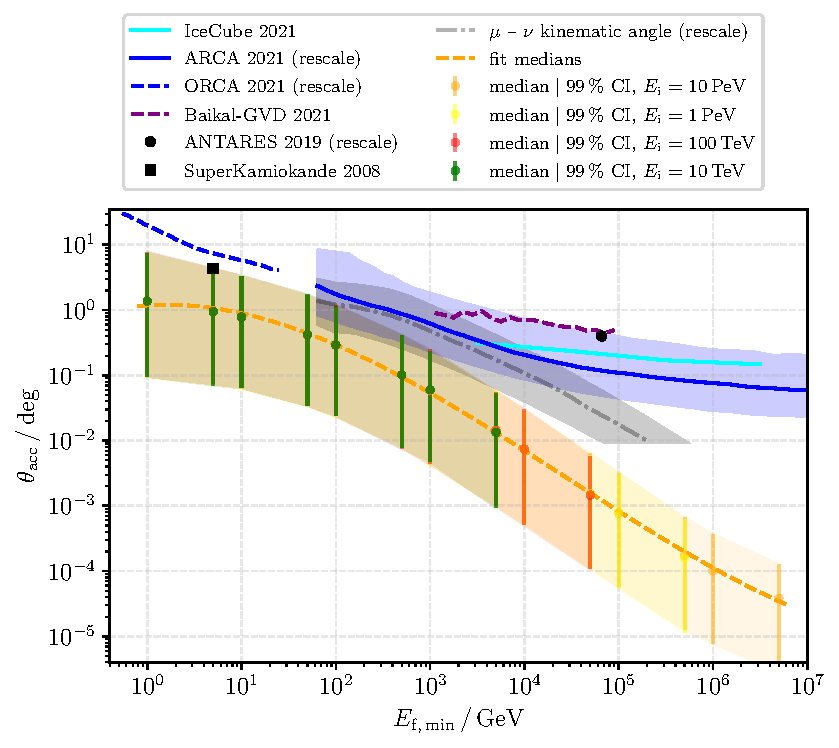
\includegraphics[width=\linewidth, height=.85\textheight, keepaspectratio]{plots/fit_median_defl_cut_10percent_only_poly_new_resolution_rescale_no_icecube_paper_final_all.pdf}
    		  \captionsetup{justification=centering}
    		  \caption*{Paper by P.~Gutjahr et al., submitted to EPJ C \\(available as \href{https://arxiv.org/abs/2208.11902}{arXiv:2208.11902})}
    		\end{figure}

        \end{column}
    \end{columns}
\end{frame}
